\documentclass[twoside]{article}

%%%%%%%%%%%%%%%%%%%%%%%%%%%%%%%%%%%%%%%%%%%%%%%%%%%%%%%%%%%%%%%%%%%%%
% Packages

\usepackage[utf8]{inputenc}

% paper settings
\usepackage{geometry}

% macro helpers
\usepackage{xspace}
\usepackage{calc}
\usepackage{ifthen}
\usepackage{amsmath}
\usepackage{listofitems}

% tabular environments
\usepackage{array}
\usepackage{multirow}

% graphics and color
\usepackage{pict2e}
\usepackage[usenames]{color}
\usepackage{colortbl}

% special symbols
\usepackage{pifont}

\usepackage{afterpage}

%--------------------------------------------------------------------
% Document-wide settings

%% paper: A5 is 148mm x 210mm
% 18mm on binding -> text area = 120mm x 190mm
\geometry{a5paper}
\geometry{portrait}
\geometry{inner=18mm,outer=10mm,top=10mm,bottom=10mm}
% Below is for lulu hardcover
%\geometry{paperheight=22.86cm,paperwidth=15.24cm}

% Don't show page numbers
\pagestyle{empty}

% Default font: Avantgarde
%\usepackage{avant}
%\renewcommand{\familydefault}{pag}
\usepackage[sfdefault]{roboto}
\usepackage[T1]{fontenc}

% no paragraph indentation
\setlength{\parindent}{0pt}

% Color definitions
% - plain black
\definecolor{Black}{gray}{0}
% - disabled days in MonthlyPlanner (from prior/next month)
\definecolor{DayMPDisabled}{gray}{0.7}
% - table headers: month names in Year Calendar and MiniCal/MonthlyPlanner
\definecolor{HeadMainBg}{gray}{0.4}
% - table second header: day names in monthy calendars (incl MiniCal/MonthlyPlanner)
\definecolor{HeadSubBg}{gray}{0.8}
% - table column color for Sat, Sun (Weekend), uncomment & tune 2nd def for color
\definecolor{WeekendDay}{gray}{0.3}
% - writing guides - primary: (thin) rules/lines, dots, etc.
\definecolor{WriteBgMain}{gray}{0.6}
% - writing guides - secondary: grey (thick) bars, etc.
\definecolor{WriteBgSec}{gray}{0.9}
% - table header background in Monthly Planner
\definecolor{HeadMainBgMP}{gray}{0.8}

% Hacks
% - required by correct \rowcolor
\setlength{\tabcolsep}{0pt}

%--------------------------------------------------------------------
% Macros

% vertical strut
%	#1 (optional) = "lift", default 0pt
%	#2            = "(total)height"
\newcommand{\vstrut}[2][0pt]{\rule[#1]{0pt}{#2}}

% Internationalization
\input{DYI_i18n}

%%%%%%%%%%%%%%%%%%%%%%%%%%%%%%%%%%%%%%%%%%%%%%%%%%%%%%%%%%%%%%%%%%%%

\input{DYI_Month_Tables.tex}
\input{DYI_Monthly_Planner_Tables.tex}

%\newcounter{DIYYear}
%\setcounter{DIYYear}{\MyYear}

\usepackage[hyphens]{url}
\usepackage{rotating}
\usepackage{forloop}% http://ctan.org/pkg/forloop
\newcounter{loopcntr}
\newcommand{\rpt}[2][1]{%
  \forloop{loopcntr}{0}{\value{loopcntr}<#1}{#2}%
}
\usepackage{tikz}
\usepackage{latexsym}
\usepackage{multicol}
\usepackage{siunitx}

\newenvironment{checklist}{%
  \begin{list}{}{}% whatever you want the list to be
  \let\olditem\item
  \renewcommand\item{\olditem[$\Box$  $\Box$] }
}{%
  \end{list}
}

\begin{document}
\setcounter{secnumdepth}{0}
\section{Founder's Journal}

Welcome to your Journal.  I designed it to help you work better.  I hope it will help you take control of your work and unlock the incredible productivity you have within by focusing your energy in the right places.
-- \textit{David Singleton, March 2016}.
\par
We recommend taking a few minutes to review the guide and videos at \linebreak\url{http://singleton.io/gettingstarted} to help you get the most out of your Journal.
\par

If you'd like to help us make the Journal better, we'd love your feedback at\linebreak \url{http://singleton.io/feedback}


\section{My Owner}

\subsection{Name}
{\color{WriteBgMain}
\rule{\textwidth}{1pt}\par}

\subsection{Contact Details}
{\color{WriteBgMain}
\rule{\textwidth}{1pt}\par
\rule{\textwidth}{1pt}\par}

%The main document needs to start on a right hand page for the weeks to lay out
%correctly
\pagebreak
This work is licensed under a Creative Commons Attribution-ShareAlike 4.0 International License.

The artwork for this journal is Based on DIY Organizer.  DIY Organizer was created by Rurik Christiansen (rurik) and is licensed under a Creative Commons License.  The source code for this version is also available under a Creative Commons License at \url{http://github.com/dps/journal}.

\pagebreak


%%%%%%%%%%%%%%%
% YEAR CALENDAR
%
% LAYOUT: 3 months per row, 4 rows (one page -- odd/right)
%					   <year>
%		---------------------------------
%		MONTH <space> MONTH <space> MONTH
%		MONTH <space> MONTH <space> MONTH
%		MONTH <space> MONTH <space> MONTH
%		MONTH <space> MONTH <space> MONTH
%		---------------------------------
%		---------------------------------
%		---------------------------------

% Settings-----------------------------------------------------------

% percentage (0.0 - 1.0) taken by the 3 months tables (3 months in a row) on the Year Calendar
% (the rest is equally split between 2 inter month-column spaces)
\newcommand\percentMonthColTWidthYC{0.95}

% calculate width of the month tabular* on the Year Calendar
\newlength{\MonthTblWidthYC}
\setlength{\MonthTblWidthYC}{( \textwidth * \real{\percentMonthColTWidthYC} ) / 3}

% calculate weekday column width inside the month tabular* on the Year Calendar
\newlength{\WkdayColWidthMonthTblYC}
\setlength{\WkdayColWidthMonthTblYC}{\MonthTblWidthYC / 7}

% Column Types for Months Tables on the Year Calendar
% Notes: - using 'tabular*' so use '@{\extracolsep\fill}')
%        - align to the 0.5em of right (supress the intercolumn space for better control)
%	 - color affects space (inserts struts in current font), put it after font change
% There are 4 types of columns
% - Column 1 (marked as weekend or weekday depending on week_starts_on_Monday value)
% This is output to DYI_i18n.tex
% - Column 2-5 (always weekday)
\newcolumntype{B}{>{\hfill\normalfont\footnotesize}p{\WkdayColWidthMonthTblYC}<{\hspace*{0.5em}}@{\extracolsep\fill}}
% - Column 6 (marked as weekend or weekday depending on week_starts_on_Monday value)
% This is output to DYI_i18n.tex
% - Column 7 (always weekend)
\newcolumntype{D}{>{\hfill\normalfont\footnotesize\color{WeekendDay}}p{\WkdayColWidthMonthTblYC}<{\hspace*{0.5em}}}

\newcommand{\MonthTblYC}[1]{%
	\begin{tabular*}{\MonthTblWidthYC}[t]{@{}A*{4}{B}CD@{}}
		\rowcolor{HeadSubBg}
		\WkdayTblRow{\bfseries\tiny} \\
		#1
	\end{tabular*}}

\newcommand{\MonthNameRowYC}[3]{%
	\rowcolor{HeadMainBg}
	\vstrut{1.1em}
	\color{white}#1 & \color{white}#2 & \color{white}#3}

% Start--------------------------------------------------------------

\hfill{\bfseries\Huge\MyYear}\par
\nointerlineskip\vspace{0.5em}
\rule{\textwidth}{1pt}

\nointerlineskip\vspace{0.5em}

\begin{tabular*}{\textwidth}{@{}>{\bfseries}c@{\extracolsep\fill}>{\bfseries}c@{\extracolsep\fill}>{\bfseries}c@{}}
	\MonthNameRowYC{\January}{\February}{\March}    \\
	\MonthTblYC{\MonthTblJan}  & \MonthTblYC{\MonthTblFeb}  & \MonthTblYC{\MonthTblMar} \\
	\MonthNameRowYC{\April}{\May}{\June}            \\
	\MonthTblYC{\MonthTblApr}  & \MonthTblYC{\MonthTblMay}  & \MonthTblYC{\MonthTblJun} \\
	\MonthNameRowYC{\July}{\August}{\September}     \\
	\MonthTblYC{\MonthTblJul}  & \MonthTblYC{\MonthTblAug}  & \MonthTblYC{\MonthTblSep} \\
	\MonthNameRowYC{\October}{\November}{\December} \\
	\MonthTblYC{\MonthTblOct}  & \MonthTblYC{\MonthTblNov}  & \MonthTblYC{\MonthTblDec}
\end{tabular*}

% fill the rest with lines, for notes
\vspace{2em}
{\color{WriteBgMain}
\rule{\textwidth}{1pt}\par
\rule{\textwidth}{1pt}\par
\rule{\textwidth}{1pt}\par
\rule{\textwidth}{1pt}\par
\rule{\textwidth}{1pt}\par
\rule{\textwidth}{1pt}\par
\rule{\textwidth}{1pt}\par
\rule{\textwidth}{1pt}\par}



\begin{figure}[!]  
\begin{center}  
\input{52wk.tex}  
\end{center}    
\end{figure}

%%%%%%%%%%%%%%%%%%%%%%%%%%%%%%%%%%%%%%%%%%%%%%%%%%%%%%%%%%%%%%%%%%%%%
%
%	MONTHLY PLANNER
%
%%%%%%%%%%%%%%%%%%%%%%%%%%%%%%%%%%%%%%%%%%%%%%%%%%%%%%%%%%%%%%%%%%%%%

% LAYOUT:       Odd Page:                   Even Page:
%		<Month>                   ||                <year>
%               --------------------------++----------------------
%               *Notes _| Mon | Tue | Wed || Thu | Fri | Sat | Sun
%		       _|     |     |     ||     |     |     |     <= 5 rows (6th will be crammed in 5th)
%               ..........................||......................
%               prior/next
%               month
%               mini cal.

% Settings-----------------------------------------------------------

% percentage (0.0 - 1.0) taken by the '*Notes' column out of the full quarter textwidth
\newcommand{\percentNoteColWidth}{0.95}
% reminder, easier to set explicitly, must add to 1.0
\newcommand{\percentNoteColWhite}{0.05}

% Column width in monthly planner: make room for rules
\newlength{\DayColWidthMP}
\setlength{\DayColWidthMP}{\textwidth / 4}

% Width of '*Notes' column
\newlength{\NoteColWidthMP}
\setlength{\NoteColWidthMP}{\DayColWidthMP * \real{\percentNoteColWidth}}
\newlength{\NoteColSkipMP}
\setlength{\NoteColSkipMP}{\DayColWidthMP * \real{\percentNoteColWhite}}

% Column Types for Days Columns in Monthly Planner
% - notes
\newcolumntype{N}{>{\centering}p{\NoteColWidthMP}@{\hspace\NoteColSkipMP}}
% - days, first/middle (Odd page: Mon, Tue; Even page: Thu, Fri, Sat)
\newcolumntype{M}{>{\centering}p{\DayColWidthMP}@{\extracolsep\fill}}
% - days, last (Odd page: Wed; Even page: Sun) \centering in combination with \\ doesn't work in last column, use \tabularnewline instead
\newcolumntype{O}{>{\centering\arraybackslash}p{\DayColWidthMP}@{}}

% Parameters for the month mini-calendars
% * Column types
\newlength{\WkdayColWidthMinicalMP}
\setlength{\WkdayColWidthMinicalMP}{\NoteColWidthMP / 7}
% There are 4 types of columns
% - Column 1 (marked as weekend or weekday depending on week_starts_on_Monday value)
% This is output to DYI_i18n.tex
% - Column 2-5 (always weekday)
\newcolumntype{F}{>{\hfill\bfseries\tiny}p{\WkdayColWidthMinicalMP}@{\extracolsep\fill}}
% - Column 6 (marked as weekend or weekday depending on week_starts_on_Monday value)
% This is output to DYI_i18n.tex
% - Column 7 (always weekend)(\vstrut is for the benefit of \color)
\newcolumntype{H}{>{\hfill\bfseries\tiny\vstrut{0pt}\color{WeekendDay}}p{\WkdayColWidthMinicalMP}}

% Tabular
\newcommand{\MonthMiniCalOnMonthlyPlanner}[2]{%
        \begin{tabular*}{\NoteColWidthMP}[t]{@{}E*{4}{F}GH@{}}
		\multicolumn{7}{>{\columncolor{HeadMainBg}}c}{\scriptsize\vstrut{1.1em}\bfseries\color{white}#1} \\
                \rowcolor{HeadSubBg}
                \WkdayTblRow{\hspace*{\fill}}\\
                #2
        \end{tabular*}}

% Notes column on odd page in Monthly Planner
% - hand tunned by trial and error, currently not posssible otherwise:
%   the heigh of the multirow is set up at the current evaluation based on current settings (font, etc)
% - so: artificially reserve (5 rows * 8 height) + 1 rows at current row heigh then build the minipage
% - last "8" reserved for building the previous/next months calendars
% Takes 4 params:
% - #1 previous month name
% - #2 previous month tabular layout
% - #3 next month name
% - #4 next month tabular layout
\newcounter{NotesColumnRows}%
\newcommand{\NoteColumn}[4]{%
	\multirow{41}{\NoteColWidthMP}{%
		\begin{minipage}{\NoteColWidthMP}%
			\makebox[0pt][l]{\smash[b]{\color{WriteBgSec}\rule[-24\baselineskip]{1em}{25\baselineskip}}}%
			{\color{WriteBgMain}\raggedright
				\setcounter{NotesColumnRows}{0}%
				\whiledo{\value{NotesColumnRows}<25}{%
					\rule{\NoteColWidthMP}{\arrayrulewidth}
					\stepcounter{NotesColumnRows}
				}%
			}%
		\end{minipage}%
		\break
		% previous month mini calendar
		\begin{minipage}{\NoteColWidthMP}%
			\renewcommand{\arraystretch}{0.8}
			\MonthMiniCalOnMonthlyPlanner{#1}{#2}
		\end{minipage}%
		\break
		% next month mini calendar
		\begin{minipage}{\NoteColWidthMP}%
			\renewcommand{\arraystretch}{0.8}
			\MonthMiniCalOnMonthlyPlanner{#3}{#4}
		\end{minipage}%
		\break \vspace{4.6pt} % push it to the top
	}%
}

% Cell format on Monthly Planner, pure play :)
% - template: #1 - color for day number and left rule, #2 - date number, #3 - holidays/text to show on date
\newcommand{\CellFormatMPTemplate}[3]{%
	% gray bar at the top, ~ half row height
	\makebox[0pt][l]{\smash[b]{\color{WriteBgSec}\rule[0.4\baselineskip]{\DayColWidthMP}{0.5\baselineskip}}}%
	% thin rule to the left almost full heigh 
	{\color{#1}\rule[-6\baselineskip]{\arrayrulewidth}{6\baselineskip}}%
	% date numbers and holiday text
	\hspace{1ex}\parbox[t]{\DayColWidthMP-1.5ex}{\color{#1}\makebox[1.7ex][r]{#2}\\\scriptsize#3}%
	% white last row, makes the left sided line open/incomplete (does not join the one below)
	\vstrut{1em}}
% this one for cramming 2 days in one table cell, for months spanning 6 rows
% - template: #1 - color for day number and left rule, #2 - first date number, #3 second date number,
% -  #4 first date holidays/text, #5 second date holidays/text
\newcommand{\CellFormatMPTemplateTwo}[5]{%
	% gray bar at the top, ~ half row height
	\makebox[0pt][l]{\smash[b]{\color{WriteBgSec}\rule[0.4\baselineskip]{\DayColWidthMP}{0.5\baselineskip}}}%
	% thin rule to the left almost full heigh 
	{\color{#1}\rule[-2.5\baselineskip]{\arrayrulewidth}{2.5\baselineskip}}%
	% date numbers and holiday text
	\hspace{1ex}\parbox[t]{\DayColWidthMP-1.5ex}{\color{#1}\makebox[1.7ex][r]{#2}\\\scriptsize#4}%
	\break%
	% white last row, makes the left sided line open/incomplete (does not join the one below)
	\vstrut{1em}%
	% repeat
	\makebox[0pt][l]{\smash[b]{\color{WriteBgSec}\rule[0.4\baselineskip]{\DayColWidthMP}{0.5\baselineskip}}}%
	{\color{#1}\rule[-2.5\baselineskip]{\arrayrulewidth}{2.5\baselineskip}}%
	\hspace{1ex}\parbox[t]{\DayColWidthMP-1.5ex}{\color{#1}\makebox[1.7ex][r]{#3}\\\scriptsize#5}%
	\break%
	\vstrut{1em}}

% for days in current month
% the optional argument is for months spanning 6 rows
\newcommand{\CellFormatMP}[4][]{%
	\ifthenelse{\equal{#1}{}}%
		{\CellFormatMPTemplate{Black}{#2}{#3}}%
		{\CellFormatMPTemplateTwo{Black}{#2}{#1}{#3}{#4}}}

% for days in previous/next month
\newcommand{\CellFormatMPDisabled}[2]{%
	\CellFormatMPTemplate{DayMPDisabled}{#1}{#2}}

% WARNING: The \vstrut in the heading for \MPLeftPage and \MPRightPage ensure enough space
%          (and proper alignmeng of the following table) when accented characters are used

% Monthly Planner Left Page
% takes 6 parameters:
% - #1   full name of current month
% - #2-5 are passed as #1-4 to \NoteColumn (see def)
% - #6   tabular layout for current month: \MP<Mon>Left
\newcommand{\MPLeftPage}[6]{%
	{\bfseries\Huge #1\vstrut[-0.5em]{1.4em}}\par
	\nointerlineskip
	\begin{tabular*}{\textwidth}{NMMO}
		\rowcolor{HeadMainBgMP}%
		% \makebox[1em] centers \ding{93} on the gray left vertical bar below, see \NoteColumn
		\bfseries\vstrut{1.1em}{\color{white}\makebox[1em]{\ding{93}}\ \ding{50}\hfill} & \bfseries\vstrut{1.1em}\color{white}\DayA & \bfseries\vstrut{1.1em}\color{white}\DayB & \bfseries\vstrut{1.1em}\color{white}\DayC \\
		% insert a dummy row: white, (cant use vspacing on previous \tabularnewline because it will turn colored as previous row)
		\\[-0.8em]
		\NoteColumn{#2}{#3}{#4}{#5}
			#6{\CellFormatMP}{\CellFormatMPDisabled}
	\end{tabular*}
	
	\clearpage
}

% Monthly Planner Right Page (similar to Right Page)
% takes 1 parameters:
% - #1    tabular layout for current month: \MP<Mon>Right
\newcommand{\MPRightPage}[1]{%
	\hfill{\bfseries\Huge\MyYear\vstrut[-0.5em]{1.4em}}\par
	\nointerlineskip

	\begin{tabular*}{\textwidth}{MMMO}
		\rowcolor{HeadMainBgMP}
		\bfseries\vstrut{1.1em}\color{white}\DayD & \bfseries\vstrut{1.1em}\color{white}\DayE & \bfseries\vstrut{1.1em}\color{white}\DayF & \bfseries\vstrut{1.1em}\color{white}\DayG \\
		% insert a dummy row: white, (cant use vspacing on previous \tabularnewline because it will turn colored as previous row)
		\\[-0.8em]
		#1{\CellFormatMP}{\CellFormatMPDisabled}
	\end{tabular*}

	\clearpage
}

\newcommand{\MyQuarter}{Q1}

\section{\MyQuarter~Objectives}
\rpt[3]{
\subsection{Objective \& Key Results}
{\color{WriteBgMain}
\rule{\textwidth}{1pt}\par
\vspace{1em}
\qquad\rule{\textwidth}{1pt}\par
\qquad\rule{\textwidth}{1pt}\par
\qquad\rule{\textwidth}{1pt}\par
\qquad\rule{\textwidth}{1pt}\par
\vspace{2em}
}
}
\let\thefootnote\relax\footnote{How to use: \url{http://singleton.io/quarterly}}
\pagebreak


\rpt[1]{
\subsection{Daily metrics}
\begin{figure}[!h]
\centering
\begin{sideways}
% GNUPLOT: LaTeX picture with Postscript
\begingroup
  \makeatletter
  \providecommand\color[2][]{%
    \GenericError{(gnuplot) \space\space\space\@spaces}{%
      Package color not loaded in conjunction with
      terminal option `colourtext'%
    }{See the gnuplot documentation for explanation.%
    }{Either use 'blacktext' in gnuplot or load the package
      color.sty in LaTeX.}%
    \renewcommand\color[2][]{}%
  }%
  \providecommand\includegraphics[2][]{%
    \GenericError{(gnuplot) \space\space\space\@spaces}{%
      Package graphicx or graphics not loaded%
    }{See the gnuplot documentation for explanation.%
    }{The gnuplot epslatex terminal needs graphicx.sty or graphics.sty.}%
    \renewcommand\includegraphics[2][]{}%
  }%
  \providecommand\rotatebox[2]{#2}%
  \@ifundefined{ifGPcolor}{%
    \newif\ifGPcolor
    \GPcolorfalse
  }{}%
  \@ifundefined{ifGPblacktext}{%
    \newif\ifGPblacktext
    \GPblacktexttrue
  }{}%
  % define a \g@addto@macro without @ in the name:
  \let\gplgaddtomacro\g@addto@macro
  % define empty templates for all commands taking text:
  \gdef\gplbacktext{}%
  \gdef\gplfronttext{}%
  \makeatother
  \ifGPblacktext
    % no textcolor at all
    \def\colorrgb#1{}%
    \def\colorgray#1{}%
  \else
    % gray or color?
    \ifGPcolor
      \def\colorrgb#1{\color[rgb]{#1}}%
      \def\colorgray#1{\color[gray]{#1}}%
      \expandafter\def\csname LTw\endcsname{\color{white}}%
      \expandafter\def\csname LTb\endcsname{\color{black}}%
      \expandafter\def\csname LTa\endcsname{\color{black}}%
      \expandafter\def\csname LT0\endcsname{\color[rgb]{1,0,0}}%
      \expandafter\def\csname LT1\endcsname{\color[rgb]{0,1,0}}%
      \expandafter\def\csname LT2\endcsname{\color[rgb]{0,0,1}}%
      \expandafter\def\csname LT3\endcsname{\color[rgb]{1,0,1}}%
      \expandafter\def\csname LT4\endcsname{\color[rgb]{0,1,1}}%
      \expandafter\def\csname LT5\endcsname{\color[rgb]{1,1,0}}%
      \expandafter\def\csname LT6\endcsname{\color[rgb]{0,0,0}}%
      \expandafter\def\csname LT7\endcsname{\color[rgb]{1,0.3,0}}%
      \expandafter\def\csname LT8\endcsname{\color[rgb]{0.5,0.5,0.5}}%
    \else
      % gray
      \def\colorrgb#1{\color{black}}%
      \def\colorgray#1{\color[gray]{#1}}%
      \expandafter\def\csname LTw\endcsname{\color{white}}%
      \expandafter\def\csname LTb\endcsname{\color{black}}%
      \expandafter\def\csname LTa\endcsname{\color{black}}%
      \expandafter\def\csname LT0\endcsname{\color{black}}%
      \expandafter\def\csname LT1\endcsname{\color{black}}%
      \expandafter\def\csname LT2\endcsname{\color{black}}%
      \expandafter\def\csname LT3\endcsname{\color{black}}%
      \expandafter\def\csname LT4\endcsname{\color{black}}%
      \expandafter\def\csname LT5\endcsname{\color{black}}%
      \expandafter\def\csname LT6\endcsname{\color{black}}%
      \expandafter\def\csname LT7\endcsname{\color{black}}%
      \expandafter\def\csname LT8\endcsname{\color{black}}%
    \fi
  \fi
    \setlength{\unitlength}{0.0500bp}%
    \ifx\gptboxheight\undefined%
      \newlength{\gptboxheight}%
      \newlength{\gptboxwidth}%
      \newsavebox{\gptboxtext}%
    \fi%
    \setlength{\fboxrule}{0.5pt}%
    \setlength{\fboxsep}{1pt}%
\begin{picture}(9354.00,6802.00)%
    \gplgaddtomacro\gplbacktext{%
      \csname LTb\endcsname%
      \put(330,704){\makebox(0,0)[r]{\strut{}$0$}}%
      \csname LTb\endcsname%
      \put(330,1287){\makebox(0,0)[r]{\strut{}$1$}}%
      \csname LTb\endcsname%
      \put(330,1871){\makebox(0,0)[r]{\strut{}$2$}}%
      \csname LTb\endcsname%
      \put(330,2454){\makebox(0,0)[r]{\strut{}$3$}}%
      \csname LTb\endcsname%
      \put(330,3037){\makebox(0,0)[r]{\strut{}$4$}}%
      \csname LTb\endcsname%
      \put(330,3621){\makebox(0,0)[r]{\strut{}$5$}}%
      \csname LTb\endcsname%
      \put(330,4204){\makebox(0,0)[r]{\strut{}$6$}}%
      \csname LTb\endcsname%
      \put(330,4787){\makebox(0,0)[r]{\strut{}$7$}}%
      \csname LTb\endcsname%
      \put(330,5370){\makebox(0,0)[r]{\strut{}$8$}}%
      \csname LTb\endcsname%
      \put(330,5954){\makebox(0,0)[r]{\strut{}$9$}}%
      \csname LTb\endcsname%
      \put(330,6537){\makebox(0,0)[r]{\strut{}$10$}}%
      \csname LTb\endcsname%
      \put(594,484){\makebox(0,0){\strut{}$0$}}%
      \csname LTb\endcsname%
      \put(1049,484){\makebox(0,0){\strut{}$5$}}%
      \csname LTb\endcsname%
      \put(1503,484){\makebox(0,0){\strut{}$10$}}%
      \csname LTb\endcsname%
      \put(1958,484){\makebox(0,0){\strut{}$15$}}%
      \csname LTb\endcsname%
      \put(2412,484){\makebox(0,0){\strut{}$20$}}%
      \csname LTb\endcsname%
      \put(2867,484){\makebox(0,0){\strut{}$25$}}%
      \csname LTb\endcsname%
      \put(3321,484){\makebox(0,0){\strut{}$30$}}%
      \csname LTb\endcsname%
      \put(3776,484){\makebox(0,0){\strut{}$35$}}%
      \csname LTb\endcsname%
      \put(4230,484){\makebox(0,0){\strut{}$40$}}%
      \csname LTb\endcsname%
      \put(4685,484){\makebox(0,0){\strut{}$45$}}%
      \csname LTb\endcsname%
      \put(5139,484){\makebox(0,0){\strut{}$50$}}%
      \csname LTb\endcsname%
      \put(5594,484){\makebox(0,0){\strut{}$55$}}%
      \csname LTb\endcsname%
      \put(6048,484){\makebox(0,0){\strut{}$60$}}%
      \csname LTb\endcsname%
      \put(6503,484){\makebox(0,0){\strut{}$65$}}%
      \csname LTb\endcsname%
      \put(6957,484){\makebox(0,0){\strut{}$70$}}%
      \csname LTb\endcsname%
      \put(7412,484){\makebox(0,0){\strut{}$75$}}%
      \csname LTb\endcsname%
      \put(7866,484){\makebox(0,0){\strut{}$80$}}%
      \csname LTb\endcsname%
      \put(8321,484){\makebox(0,0){\strut{}$85$}}%
      \csname LTb\endcsname%
      \put(8775,484){\makebox(0,0){\strut{}$90$}}%
    }%
    \gplgaddtomacro\gplfronttext{%
      \csname LTb\endcsname%
      \put(4775,154){\makebox(0,0){\strut{}day of quarter}}%
      \put(4775,6427){\makebox(0,0){\strut{}}}%
    }%
    \gplbacktext
    \put(0,0){\includegraphics{daily}}%
    \gplfronttext
  \end{picture}%
\endgroup

\end{sideways}
\end{figure}
\let\thefootnote\relax\footnote{How to use: \url{http://singleton.io/daily}}
\pagebreak
}

% Start--------------------------------------------------------------

\MPLeftPage{\January}{\December}{\MonthTblDecPrev}{\February}{\MonthTblFeb}{\MPJanLeft}
\MPRightPage{\MPJanRight}

\MPLeftPage{\February}{\January}{\MonthTblJan}{\March}{\MonthTblMar}{\MPFebLeft}
\MPRightPage{\MPFebRight}

\MPLeftPage{\March}{\February}{\MonthTblFeb}{\April}{\MonthTblApr}{\MPMarLeft}
\MPRightPage{\MPMarRight}

\renewcommand{\MyQuarter}{Q2}

\section{\MyQuarter~Objectives}
\rpt[3]{
\subsection{Objective \& Key Results}
{\color{WriteBgMain}
\rule{\textwidth}{1pt}\par
\vspace{1em}
\qquad\rule{\textwidth}{1pt}\par
\qquad\rule{\textwidth}{1pt}\par
\qquad\rule{\textwidth}{1pt}\par
\qquad\rule{\textwidth}{1pt}\par
\vspace{2em}
}
}
\let\thefootnote\relax\footnote{How to use: \url{http://singleton.io/quarterly}}
\pagebreak


\rpt[1]{
\subsection{Daily metrics}
\begin{figure}[!h]
\centering
\begin{sideways}
% GNUPLOT: LaTeX picture with Postscript
\begingroup
  \makeatletter
  \providecommand\color[2][]{%
    \GenericError{(gnuplot) \space\space\space\@spaces}{%
      Package color not loaded in conjunction with
      terminal option `colourtext'%
    }{See the gnuplot documentation for explanation.%
    }{Either use 'blacktext' in gnuplot or load the package
      color.sty in LaTeX.}%
    \renewcommand\color[2][]{}%
  }%
  \providecommand\includegraphics[2][]{%
    \GenericError{(gnuplot) \space\space\space\@spaces}{%
      Package graphicx or graphics not loaded%
    }{See the gnuplot documentation for explanation.%
    }{The gnuplot epslatex terminal needs graphicx.sty or graphics.sty.}%
    \renewcommand\includegraphics[2][]{}%
  }%
  \providecommand\rotatebox[2]{#2}%
  \@ifundefined{ifGPcolor}{%
    \newif\ifGPcolor
    \GPcolorfalse
  }{}%
  \@ifundefined{ifGPblacktext}{%
    \newif\ifGPblacktext
    \GPblacktexttrue
  }{}%
  % define a \g@addto@macro without @ in the name:
  \let\gplgaddtomacro\g@addto@macro
  % define empty templates for all commands taking text:
  \gdef\gplbacktext{}%
  \gdef\gplfronttext{}%
  \makeatother
  \ifGPblacktext
    % no textcolor at all
    \def\colorrgb#1{}%
    \def\colorgray#1{}%
  \else
    % gray or color?
    \ifGPcolor
      \def\colorrgb#1{\color[rgb]{#1}}%
      \def\colorgray#1{\color[gray]{#1}}%
      \expandafter\def\csname LTw\endcsname{\color{white}}%
      \expandafter\def\csname LTb\endcsname{\color{black}}%
      \expandafter\def\csname LTa\endcsname{\color{black}}%
      \expandafter\def\csname LT0\endcsname{\color[rgb]{1,0,0}}%
      \expandafter\def\csname LT1\endcsname{\color[rgb]{0,1,0}}%
      \expandafter\def\csname LT2\endcsname{\color[rgb]{0,0,1}}%
      \expandafter\def\csname LT3\endcsname{\color[rgb]{1,0,1}}%
      \expandafter\def\csname LT4\endcsname{\color[rgb]{0,1,1}}%
      \expandafter\def\csname LT5\endcsname{\color[rgb]{1,1,0}}%
      \expandafter\def\csname LT6\endcsname{\color[rgb]{0,0,0}}%
      \expandafter\def\csname LT7\endcsname{\color[rgb]{1,0.3,0}}%
      \expandafter\def\csname LT8\endcsname{\color[rgb]{0.5,0.5,0.5}}%
    \else
      % gray
      \def\colorrgb#1{\color{black}}%
      \def\colorgray#1{\color[gray]{#1}}%
      \expandafter\def\csname LTw\endcsname{\color{white}}%
      \expandafter\def\csname LTb\endcsname{\color{black}}%
      \expandafter\def\csname LTa\endcsname{\color{black}}%
      \expandafter\def\csname LT0\endcsname{\color{black}}%
      \expandafter\def\csname LT1\endcsname{\color{black}}%
      \expandafter\def\csname LT2\endcsname{\color{black}}%
      \expandafter\def\csname LT3\endcsname{\color{black}}%
      \expandafter\def\csname LT4\endcsname{\color{black}}%
      \expandafter\def\csname LT5\endcsname{\color{black}}%
      \expandafter\def\csname LT6\endcsname{\color{black}}%
      \expandafter\def\csname LT7\endcsname{\color{black}}%
      \expandafter\def\csname LT8\endcsname{\color{black}}%
    \fi
  \fi
    \setlength{\unitlength}{0.0500bp}%
    \ifx\gptboxheight\undefined%
      \newlength{\gptboxheight}%
      \newlength{\gptboxwidth}%
      \newsavebox{\gptboxtext}%
    \fi%
    \setlength{\fboxrule}{0.5pt}%
    \setlength{\fboxsep}{1pt}%
\begin{picture}(9354.00,6802.00)%
    \gplgaddtomacro\gplbacktext{%
      \csname LTb\endcsname%
      \put(330,704){\makebox(0,0)[r]{\strut{}$0$}}%
      \csname LTb\endcsname%
      \put(330,1287){\makebox(0,0)[r]{\strut{}$1$}}%
      \csname LTb\endcsname%
      \put(330,1871){\makebox(0,0)[r]{\strut{}$2$}}%
      \csname LTb\endcsname%
      \put(330,2454){\makebox(0,0)[r]{\strut{}$3$}}%
      \csname LTb\endcsname%
      \put(330,3037){\makebox(0,0)[r]{\strut{}$4$}}%
      \csname LTb\endcsname%
      \put(330,3621){\makebox(0,0)[r]{\strut{}$5$}}%
      \csname LTb\endcsname%
      \put(330,4204){\makebox(0,0)[r]{\strut{}$6$}}%
      \csname LTb\endcsname%
      \put(330,4787){\makebox(0,0)[r]{\strut{}$7$}}%
      \csname LTb\endcsname%
      \put(330,5370){\makebox(0,0)[r]{\strut{}$8$}}%
      \csname LTb\endcsname%
      \put(330,5954){\makebox(0,0)[r]{\strut{}$9$}}%
      \csname LTb\endcsname%
      \put(330,6537){\makebox(0,0)[r]{\strut{}$10$}}%
      \csname LTb\endcsname%
      \put(594,484){\makebox(0,0){\strut{}$0$}}%
      \csname LTb\endcsname%
      \put(1049,484){\makebox(0,0){\strut{}$5$}}%
      \csname LTb\endcsname%
      \put(1503,484){\makebox(0,0){\strut{}$10$}}%
      \csname LTb\endcsname%
      \put(1958,484){\makebox(0,0){\strut{}$15$}}%
      \csname LTb\endcsname%
      \put(2412,484){\makebox(0,0){\strut{}$20$}}%
      \csname LTb\endcsname%
      \put(2867,484){\makebox(0,0){\strut{}$25$}}%
      \csname LTb\endcsname%
      \put(3321,484){\makebox(0,0){\strut{}$30$}}%
      \csname LTb\endcsname%
      \put(3776,484){\makebox(0,0){\strut{}$35$}}%
      \csname LTb\endcsname%
      \put(4230,484){\makebox(0,0){\strut{}$40$}}%
      \csname LTb\endcsname%
      \put(4685,484){\makebox(0,0){\strut{}$45$}}%
      \csname LTb\endcsname%
      \put(5139,484){\makebox(0,0){\strut{}$50$}}%
      \csname LTb\endcsname%
      \put(5594,484){\makebox(0,0){\strut{}$55$}}%
      \csname LTb\endcsname%
      \put(6048,484){\makebox(0,0){\strut{}$60$}}%
      \csname LTb\endcsname%
      \put(6503,484){\makebox(0,0){\strut{}$65$}}%
      \csname LTb\endcsname%
      \put(6957,484){\makebox(0,0){\strut{}$70$}}%
      \csname LTb\endcsname%
      \put(7412,484){\makebox(0,0){\strut{}$75$}}%
      \csname LTb\endcsname%
      \put(7866,484){\makebox(0,0){\strut{}$80$}}%
      \csname LTb\endcsname%
      \put(8321,484){\makebox(0,0){\strut{}$85$}}%
      \csname LTb\endcsname%
      \put(8775,484){\makebox(0,0){\strut{}$90$}}%
    }%
    \gplgaddtomacro\gplfronttext{%
      \csname LTb\endcsname%
      \put(4775,154){\makebox(0,0){\strut{}day of quarter}}%
      \put(4775,6427){\makebox(0,0){\strut{}}}%
    }%
    \gplbacktext
    \put(0,0){\includegraphics{daily}}%
    \gplfronttext
  \end{picture}%
\endgroup

\end{sideways}
\end{figure}
\let\thefootnote\relax\footnote{How to use: \url{http://singleton.io/daily}}
\pagebreak
}


\MPLeftPage{\April}{\March}{\MonthTblMar}{\May}{\MonthTblMay}{\MPAprLeft}
\MPRightPage{\MPAprRight}

\MPLeftPage{\May}{\April}{\MonthTblApr}{\June}{\MonthTblJun}{\MPMayLeft}
\MPRightPage{\MPMayRight}

\MPLeftPage{\June}{\May}{\MonthTblMay}{\July}{\MonthTblJul}{\MPJunLeft}
\MPRightPage{\MPJunRight}

\renewcommand{\MyQuarter}{Q3}

\section{\MyQuarter~Objectives}
\rpt[3]{
\subsection{Objective \& Key Results}
{\color{WriteBgMain}
\rule{\textwidth}{1pt}\par
\vspace{1em}
\qquad\rule{\textwidth}{1pt}\par
\qquad\rule{\textwidth}{1pt}\par
\qquad\rule{\textwidth}{1pt}\par
\qquad\rule{\textwidth}{1pt}\par
\vspace{2em}
}
}
\let\thefootnote\relax\footnote{How to use: \url{http://singleton.io/quarterly}}
\pagebreak


\rpt[1]{
\subsection{Daily metrics}
\begin{figure}[!h]
\centering
\begin{sideways}
% GNUPLOT: LaTeX picture with Postscript
\begingroup
  \makeatletter
  \providecommand\color[2][]{%
    \GenericError{(gnuplot) \space\space\space\@spaces}{%
      Package color not loaded in conjunction with
      terminal option `colourtext'%
    }{See the gnuplot documentation for explanation.%
    }{Either use 'blacktext' in gnuplot or load the package
      color.sty in LaTeX.}%
    \renewcommand\color[2][]{}%
  }%
  \providecommand\includegraphics[2][]{%
    \GenericError{(gnuplot) \space\space\space\@spaces}{%
      Package graphicx or graphics not loaded%
    }{See the gnuplot documentation for explanation.%
    }{The gnuplot epslatex terminal needs graphicx.sty or graphics.sty.}%
    \renewcommand\includegraphics[2][]{}%
  }%
  \providecommand\rotatebox[2]{#2}%
  \@ifundefined{ifGPcolor}{%
    \newif\ifGPcolor
    \GPcolorfalse
  }{}%
  \@ifundefined{ifGPblacktext}{%
    \newif\ifGPblacktext
    \GPblacktexttrue
  }{}%
  % define a \g@addto@macro without @ in the name:
  \let\gplgaddtomacro\g@addto@macro
  % define empty templates for all commands taking text:
  \gdef\gplbacktext{}%
  \gdef\gplfronttext{}%
  \makeatother
  \ifGPblacktext
    % no textcolor at all
    \def\colorrgb#1{}%
    \def\colorgray#1{}%
  \else
    % gray or color?
    \ifGPcolor
      \def\colorrgb#1{\color[rgb]{#1}}%
      \def\colorgray#1{\color[gray]{#1}}%
      \expandafter\def\csname LTw\endcsname{\color{white}}%
      \expandafter\def\csname LTb\endcsname{\color{black}}%
      \expandafter\def\csname LTa\endcsname{\color{black}}%
      \expandafter\def\csname LT0\endcsname{\color[rgb]{1,0,0}}%
      \expandafter\def\csname LT1\endcsname{\color[rgb]{0,1,0}}%
      \expandafter\def\csname LT2\endcsname{\color[rgb]{0,0,1}}%
      \expandafter\def\csname LT3\endcsname{\color[rgb]{1,0,1}}%
      \expandafter\def\csname LT4\endcsname{\color[rgb]{0,1,1}}%
      \expandafter\def\csname LT5\endcsname{\color[rgb]{1,1,0}}%
      \expandafter\def\csname LT6\endcsname{\color[rgb]{0,0,0}}%
      \expandafter\def\csname LT7\endcsname{\color[rgb]{1,0.3,0}}%
      \expandafter\def\csname LT8\endcsname{\color[rgb]{0.5,0.5,0.5}}%
    \else
      % gray
      \def\colorrgb#1{\color{black}}%
      \def\colorgray#1{\color[gray]{#1}}%
      \expandafter\def\csname LTw\endcsname{\color{white}}%
      \expandafter\def\csname LTb\endcsname{\color{black}}%
      \expandafter\def\csname LTa\endcsname{\color{black}}%
      \expandafter\def\csname LT0\endcsname{\color{black}}%
      \expandafter\def\csname LT1\endcsname{\color{black}}%
      \expandafter\def\csname LT2\endcsname{\color{black}}%
      \expandafter\def\csname LT3\endcsname{\color{black}}%
      \expandafter\def\csname LT4\endcsname{\color{black}}%
      \expandafter\def\csname LT5\endcsname{\color{black}}%
      \expandafter\def\csname LT6\endcsname{\color{black}}%
      \expandafter\def\csname LT7\endcsname{\color{black}}%
      \expandafter\def\csname LT8\endcsname{\color{black}}%
    \fi
  \fi
    \setlength{\unitlength}{0.0500bp}%
    \ifx\gptboxheight\undefined%
      \newlength{\gptboxheight}%
      \newlength{\gptboxwidth}%
      \newsavebox{\gptboxtext}%
    \fi%
    \setlength{\fboxrule}{0.5pt}%
    \setlength{\fboxsep}{1pt}%
\begin{picture}(9354.00,6802.00)%
    \gplgaddtomacro\gplbacktext{%
      \csname LTb\endcsname%
      \put(330,704){\makebox(0,0)[r]{\strut{}$0$}}%
      \csname LTb\endcsname%
      \put(330,1287){\makebox(0,0)[r]{\strut{}$1$}}%
      \csname LTb\endcsname%
      \put(330,1871){\makebox(0,0)[r]{\strut{}$2$}}%
      \csname LTb\endcsname%
      \put(330,2454){\makebox(0,0)[r]{\strut{}$3$}}%
      \csname LTb\endcsname%
      \put(330,3037){\makebox(0,0)[r]{\strut{}$4$}}%
      \csname LTb\endcsname%
      \put(330,3621){\makebox(0,0)[r]{\strut{}$5$}}%
      \csname LTb\endcsname%
      \put(330,4204){\makebox(0,0)[r]{\strut{}$6$}}%
      \csname LTb\endcsname%
      \put(330,4787){\makebox(0,0)[r]{\strut{}$7$}}%
      \csname LTb\endcsname%
      \put(330,5370){\makebox(0,0)[r]{\strut{}$8$}}%
      \csname LTb\endcsname%
      \put(330,5954){\makebox(0,0)[r]{\strut{}$9$}}%
      \csname LTb\endcsname%
      \put(330,6537){\makebox(0,0)[r]{\strut{}$10$}}%
      \csname LTb\endcsname%
      \put(594,484){\makebox(0,0){\strut{}$0$}}%
      \csname LTb\endcsname%
      \put(1049,484){\makebox(0,0){\strut{}$5$}}%
      \csname LTb\endcsname%
      \put(1503,484){\makebox(0,0){\strut{}$10$}}%
      \csname LTb\endcsname%
      \put(1958,484){\makebox(0,0){\strut{}$15$}}%
      \csname LTb\endcsname%
      \put(2412,484){\makebox(0,0){\strut{}$20$}}%
      \csname LTb\endcsname%
      \put(2867,484){\makebox(0,0){\strut{}$25$}}%
      \csname LTb\endcsname%
      \put(3321,484){\makebox(0,0){\strut{}$30$}}%
      \csname LTb\endcsname%
      \put(3776,484){\makebox(0,0){\strut{}$35$}}%
      \csname LTb\endcsname%
      \put(4230,484){\makebox(0,0){\strut{}$40$}}%
      \csname LTb\endcsname%
      \put(4685,484){\makebox(0,0){\strut{}$45$}}%
      \csname LTb\endcsname%
      \put(5139,484){\makebox(0,0){\strut{}$50$}}%
      \csname LTb\endcsname%
      \put(5594,484){\makebox(0,0){\strut{}$55$}}%
      \csname LTb\endcsname%
      \put(6048,484){\makebox(0,0){\strut{}$60$}}%
      \csname LTb\endcsname%
      \put(6503,484){\makebox(0,0){\strut{}$65$}}%
      \csname LTb\endcsname%
      \put(6957,484){\makebox(0,0){\strut{}$70$}}%
      \csname LTb\endcsname%
      \put(7412,484){\makebox(0,0){\strut{}$75$}}%
      \csname LTb\endcsname%
      \put(7866,484){\makebox(0,0){\strut{}$80$}}%
      \csname LTb\endcsname%
      \put(8321,484){\makebox(0,0){\strut{}$85$}}%
      \csname LTb\endcsname%
      \put(8775,484){\makebox(0,0){\strut{}$90$}}%
    }%
    \gplgaddtomacro\gplfronttext{%
      \csname LTb\endcsname%
      \put(4775,154){\makebox(0,0){\strut{}day of quarter}}%
      \put(4775,6427){\makebox(0,0){\strut{}}}%
    }%
    \gplbacktext
    \put(0,0){\includegraphics{daily}}%
    \gplfronttext
  \end{picture}%
\endgroup

\end{sideways}
\end{figure}
\let\thefootnote\relax\footnote{How to use: \url{http://singleton.io/daily}}
\pagebreak
}


\MPLeftPage{\July}{\June}{\MonthTblJun}{\August}{\MonthTblAug}{\MPJulLeft}
\MPRightPage{\MPJulRight}

\MPLeftPage{\August}{\July}{\MonthTblJul}{\September}{\MonthTblSep}{\MPAugLeft}
\MPRightPage{\MPAugRight}

\MPLeftPage{\September}{\August}{\MonthTblAug}{\October}{\MonthTblOct}{\MPSepLeft}
\MPRightPage{\MPSepRight}

\renewcommand{\MyQuarter}{Q4}

\section{\MyQuarter~Objectives}
\rpt[3]{
\subsection{Objective \& Key Results}
{\color{WriteBgMain}
\rule{\textwidth}{1pt}\par
\vspace{1em}
\qquad\rule{\textwidth}{1pt}\par
\qquad\rule{\textwidth}{1pt}\par
\qquad\rule{\textwidth}{1pt}\par
\qquad\rule{\textwidth}{1pt}\par
\vspace{2em}
}
}
\let\thefootnote\relax\footnote{How to use: \url{http://singleton.io/quarterly}}
\pagebreak


\rpt[1]{
\subsection{Daily metrics}
\begin{figure}[!h]
\centering
\begin{sideways}
% GNUPLOT: LaTeX picture with Postscript
\begingroup
  \makeatletter
  \providecommand\color[2][]{%
    \GenericError{(gnuplot) \space\space\space\@spaces}{%
      Package color not loaded in conjunction with
      terminal option `colourtext'%
    }{See the gnuplot documentation for explanation.%
    }{Either use 'blacktext' in gnuplot or load the package
      color.sty in LaTeX.}%
    \renewcommand\color[2][]{}%
  }%
  \providecommand\includegraphics[2][]{%
    \GenericError{(gnuplot) \space\space\space\@spaces}{%
      Package graphicx or graphics not loaded%
    }{See the gnuplot documentation for explanation.%
    }{The gnuplot epslatex terminal needs graphicx.sty or graphics.sty.}%
    \renewcommand\includegraphics[2][]{}%
  }%
  \providecommand\rotatebox[2]{#2}%
  \@ifundefined{ifGPcolor}{%
    \newif\ifGPcolor
    \GPcolorfalse
  }{}%
  \@ifundefined{ifGPblacktext}{%
    \newif\ifGPblacktext
    \GPblacktexttrue
  }{}%
  % define a \g@addto@macro without @ in the name:
  \let\gplgaddtomacro\g@addto@macro
  % define empty templates for all commands taking text:
  \gdef\gplbacktext{}%
  \gdef\gplfronttext{}%
  \makeatother
  \ifGPblacktext
    % no textcolor at all
    \def\colorrgb#1{}%
    \def\colorgray#1{}%
  \else
    % gray or color?
    \ifGPcolor
      \def\colorrgb#1{\color[rgb]{#1}}%
      \def\colorgray#1{\color[gray]{#1}}%
      \expandafter\def\csname LTw\endcsname{\color{white}}%
      \expandafter\def\csname LTb\endcsname{\color{black}}%
      \expandafter\def\csname LTa\endcsname{\color{black}}%
      \expandafter\def\csname LT0\endcsname{\color[rgb]{1,0,0}}%
      \expandafter\def\csname LT1\endcsname{\color[rgb]{0,1,0}}%
      \expandafter\def\csname LT2\endcsname{\color[rgb]{0,0,1}}%
      \expandafter\def\csname LT3\endcsname{\color[rgb]{1,0,1}}%
      \expandafter\def\csname LT4\endcsname{\color[rgb]{0,1,1}}%
      \expandafter\def\csname LT5\endcsname{\color[rgb]{1,1,0}}%
      \expandafter\def\csname LT6\endcsname{\color[rgb]{0,0,0}}%
      \expandafter\def\csname LT7\endcsname{\color[rgb]{1,0.3,0}}%
      \expandafter\def\csname LT8\endcsname{\color[rgb]{0.5,0.5,0.5}}%
    \else
      % gray
      \def\colorrgb#1{\color{black}}%
      \def\colorgray#1{\color[gray]{#1}}%
      \expandafter\def\csname LTw\endcsname{\color{white}}%
      \expandafter\def\csname LTb\endcsname{\color{black}}%
      \expandafter\def\csname LTa\endcsname{\color{black}}%
      \expandafter\def\csname LT0\endcsname{\color{black}}%
      \expandafter\def\csname LT1\endcsname{\color{black}}%
      \expandafter\def\csname LT2\endcsname{\color{black}}%
      \expandafter\def\csname LT3\endcsname{\color{black}}%
      \expandafter\def\csname LT4\endcsname{\color{black}}%
      \expandafter\def\csname LT5\endcsname{\color{black}}%
      \expandafter\def\csname LT6\endcsname{\color{black}}%
      \expandafter\def\csname LT7\endcsname{\color{black}}%
      \expandafter\def\csname LT8\endcsname{\color{black}}%
    \fi
  \fi
    \setlength{\unitlength}{0.0500bp}%
    \ifx\gptboxheight\undefined%
      \newlength{\gptboxheight}%
      \newlength{\gptboxwidth}%
      \newsavebox{\gptboxtext}%
    \fi%
    \setlength{\fboxrule}{0.5pt}%
    \setlength{\fboxsep}{1pt}%
\begin{picture}(9354.00,6802.00)%
    \gplgaddtomacro\gplbacktext{%
      \csname LTb\endcsname%
      \put(330,704){\makebox(0,0)[r]{\strut{}$0$}}%
      \csname LTb\endcsname%
      \put(330,1287){\makebox(0,0)[r]{\strut{}$1$}}%
      \csname LTb\endcsname%
      \put(330,1871){\makebox(0,0)[r]{\strut{}$2$}}%
      \csname LTb\endcsname%
      \put(330,2454){\makebox(0,0)[r]{\strut{}$3$}}%
      \csname LTb\endcsname%
      \put(330,3037){\makebox(0,0)[r]{\strut{}$4$}}%
      \csname LTb\endcsname%
      \put(330,3621){\makebox(0,0)[r]{\strut{}$5$}}%
      \csname LTb\endcsname%
      \put(330,4204){\makebox(0,0)[r]{\strut{}$6$}}%
      \csname LTb\endcsname%
      \put(330,4787){\makebox(0,0)[r]{\strut{}$7$}}%
      \csname LTb\endcsname%
      \put(330,5370){\makebox(0,0)[r]{\strut{}$8$}}%
      \csname LTb\endcsname%
      \put(330,5954){\makebox(0,0)[r]{\strut{}$9$}}%
      \csname LTb\endcsname%
      \put(330,6537){\makebox(0,0)[r]{\strut{}$10$}}%
      \csname LTb\endcsname%
      \put(594,484){\makebox(0,0){\strut{}$0$}}%
      \csname LTb\endcsname%
      \put(1049,484){\makebox(0,0){\strut{}$5$}}%
      \csname LTb\endcsname%
      \put(1503,484){\makebox(0,0){\strut{}$10$}}%
      \csname LTb\endcsname%
      \put(1958,484){\makebox(0,0){\strut{}$15$}}%
      \csname LTb\endcsname%
      \put(2412,484){\makebox(0,0){\strut{}$20$}}%
      \csname LTb\endcsname%
      \put(2867,484){\makebox(0,0){\strut{}$25$}}%
      \csname LTb\endcsname%
      \put(3321,484){\makebox(0,0){\strut{}$30$}}%
      \csname LTb\endcsname%
      \put(3776,484){\makebox(0,0){\strut{}$35$}}%
      \csname LTb\endcsname%
      \put(4230,484){\makebox(0,0){\strut{}$40$}}%
      \csname LTb\endcsname%
      \put(4685,484){\makebox(0,0){\strut{}$45$}}%
      \csname LTb\endcsname%
      \put(5139,484){\makebox(0,0){\strut{}$50$}}%
      \csname LTb\endcsname%
      \put(5594,484){\makebox(0,0){\strut{}$55$}}%
      \csname LTb\endcsname%
      \put(6048,484){\makebox(0,0){\strut{}$60$}}%
      \csname LTb\endcsname%
      \put(6503,484){\makebox(0,0){\strut{}$65$}}%
      \csname LTb\endcsname%
      \put(6957,484){\makebox(0,0){\strut{}$70$}}%
      \csname LTb\endcsname%
      \put(7412,484){\makebox(0,0){\strut{}$75$}}%
      \csname LTb\endcsname%
      \put(7866,484){\makebox(0,0){\strut{}$80$}}%
      \csname LTb\endcsname%
      \put(8321,484){\makebox(0,0){\strut{}$85$}}%
      \csname LTb\endcsname%
      \put(8775,484){\makebox(0,0){\strut{}$90$}}%
    }%
    \gplgaddtomacro\gplfronttext{%
      \csname LTb\endcsname%
      \put(4775,154){\makebox(0,0){\strut{}day of quarter}}%
      \put(4775,6427){\makebox(0,0){\strut{}}}%
    }%
    \gplbacktext
    \put(0,0){\includegraphics{daily}}%
    \gplfronttext
  \end{picture}%
\endgroup

\end{sideways}
\end{figure}
\let\thefootnote\relax\footnote{How to use: \url{http://singleton.io/daily}}
\pagebreak
}


\MPLeftPage{\October}{\September}{\MonthTblSep}{\November}{\MonthTblNov}{\MPOctLeft}
\MPRightPage{\MPOctRight}

\MPLeftPage{\November}{\October}{\MonthTblOct}{\December}{\MonthTblDec}{\MPNovLeft}
\MPRightPage{\MPNovRight}

\MPLeftPage{\December}{\November}{\MonthTblNov}{\January}{\MonthTblJanNext}{\MPDecLeft}
\MPRightPage{\MPDecRight}



%%%%%%%%%%%%%%%%%%%%%%%%%%%%%%%%%%%%%%%%%%%%%%%%%%%%%%%%%%%%%%%%%%%%%
%
%       WEERKLY PLANNER
%
%%%%%%%%%%%%%%%%%%%%%%%%%%%%%%%%%%%%%%%%%%%%%%%%%%%%%%%%%%%%%%%%%%%%%

% LAYOUT: Odd Page                          Even Page
%         Week <N>                             <Month> <Year>
%         Week Goals                [Notes] || Thursday Day Month(abbr) [Notes]
%         Monday Day Month(abbr)    [Notes] || Friday Day Month(abbr)   [Notes]
%         Tuesday Day Month(abbr)   [     ] || Saturday& Sunday Day Month(abbr) [  ]
%         Wednesday Day Month(abbr) [     ] || How did it go?   [     ]

% Settings-----------------------------------------------------------

% Space partitioning
% - space for the hour entry at the beginning of the filler row
\newlength{\HourBondingBoxWP}
\setlength{\HourBondingBoxWP}{2.5ex}
%   |<--textwidth-------------------------------------------------------------------------------->|
%   |<--DayFillerTotWidthWP------------------------------------------>|<--NotesFillerTotWidthWP-->|
%   |<--DayFillerWidthWP-------------------------->|<-DayFillerSepWP->|<--NotesFillerTotWidthWP-->|
%   |<-HourBondingBoxWP->|<-DayFillerRulerWidthWP->|<-DayFillerSepWP->|<--NotesFillerTotWidthWP-->|
\newlength{\DayFillerTotWidthWP}
\setlength{\DayFillerTotWidthWP}{( \textwidth ) /2}
\newlength{\DayFillerThirdTotWidthWP}
\setlength{\DayFillerThirdTotWidthWP}{( \textwidth ) / 3}
\newlength{\DayFillerSixthTotWidthWP}
\setlength{\DayFillerSixthTotWidthWP}{( \textwidth ) / 6}

\newlength{\DayFillerSepWP}
\setlength{\DayFillerSepWP}{1em}
\newlength{\DayFillerWidthWP}
\setlength{\DayFillerWidthWP}{\DayFillerTotWidthWP - \DayFillerSepWP}
\newlength{\DayFillerThirdWidthWP}
\setlength{\DayFillerThirdWidthWP}{\DayFillerThirdTotWidthWP - \DayFillerSepWP}
\newlength{\DayFillerSixthWidthWP}
\setlength{\DayFillerSixthWidthWP}{\DayFillerSixthTotWidthWP - \DayFillerSepWP}

\newlength{\DayFillerRulerWidthWP}
\setlength{\DayFillerRulerWidthWP}{\DayFillerWidthWP - \HourBondingBoxWP}
\newlength{\NotesFillerTotWidthWP}
\setlength{\NotesFillerTotWidthWP}{\textwidth - \DayFillerTotWidthWP}
% minicalendar space partitioning
%   |<-DayFillerWidthWP-------------------------------------->|
%   |<-PrevMonth->|<-sep->|<-CurrMonth->|<-sep->|<-NextMonth->|
\newlength{\MinicalSepWP}
\setlength{\MinicalSepWP}{2ex}
\newlength{\MinicalWidthWP}
\setlength{\MinicalWidthWP}{( \DayFillerWidthWP - 2 \MinicalSepWP ) / 3}
%   column width in Minical
\newlength{\MinicalColWidthWP}
\setlength{\MinicalColWidthWP}{\MinicalWidthWP / 7}

% Day entry contents on Weekly Planner
% - one row:
%   <hour>________<-sep->___
%   (#1 is the current hour, right aligned inside a makebox,  also using a vstrut to define heigh
\newcommand{\DayFillerRowWP}[2]{%
	\makebox[\HourBondingBoxWP]{\hspace{\fill}#1\hspace{0.5em}}\vstrut{11.5pt}{\color{Black}\raisebox{.2ex}{\rlap{#2}}\color{WriteBgMain}\rule{\DayFillerRulerWidthWP}{0.5pt}}%
	\hspace*{\DayFillerSepWP}%
	{\color{WriteBgMain}\rule{\NotesFillerTotWidthWP}{0.5pt}}}
% - as above but no <hour>
\newcommand{\DayFillerRowEWP}{%
	\vstrut{11.5pt}%
        {\color{WriteBgMain}\rule{\DayFillerWidthWP}{0.5pt}}%
        \hspace*{\DayFillerSepWP}%
        {\color{WriteBgMain}\rule{\NotesFillerTotWidthWP}{0.5pt}}}
% - then fill, with hour intervals
\newcommand{\DayFillerWP}[1]{%
    \setsepchar{\\}%
    \readlist*\parsed{#1\\\\\\\\\\\\\\}% Need enough separators to get all of our lines
	\DayFillerRowWP{\ding{46}}{\parsed[1]}\break%
	\DayFillerRowWP{}{\parsed[2]}\break%
	\DayFillerRowWP{}{\parsed[3]}\break%
	\DayFillerRowWP{}{\parsed[4]}\break%
	\DayFillerRowWP{}{\parsed[5]}\break%
	\DayFillerRowWP{}{\parsed[6]}\break%
	\DayFillerRowWP{}{\parsed[7]}\break%
	\DayFillerRowWP{}{\parsed[8]}}

% Monthly minicalendars on Weekly Planner
% Column types I,J,K
% - weeekdays
\newcolumntype{I}{>{\hfill\bfseries\tiny}p{\MinicalColWidthWP}@{\extracolsep\fill}}
% - Saturday
\newcolumntype{J}{>{\hfill\bfseries\tiny\vstrut{0pt}\color{WeekendDay}}p{\MinicalColWidthWP}@{\extracolsep\fill}}
% - Sunday (last column)
\newcolumntype{K}{>{\hfill\bfseries\tiny\vstrut{0pt}\color{WeekendDay}}p{\MinicalColWidthWP}}
% - Monthly Minicals, center the weekdays headline
\newcommand{\myCentering}[1]{\hspace*{\fill}#1\hspace*{\fill}}
\newcommand{\MonthMiniCalWP}[2]{%
	{\renewcommand{\arraystretch}{0.6}%
	\begin{tabular*}{\MinicalWidthWP}[t]{@{}*{5}{I}JK@{}}
	\multicolumn{7}{>{\columncolor{HeadMainBg}}c}{\scriptsize\vstrut{1.1em}\bfseries\color{white}#1} \\
	\rowcolor{HeadSubBg}%
	\WkdayTblRowA{\myCentering} \\
	#2
	\end{tabular*}}}

% Day entry in Weekly Planner
\newcommand{\DayWP}[2]{%
	% gray shading bar
	\makebox[0pt][l]{\smash[b]{\color{WriteBgSec}\rule[0.4\baselineskip]{\DayFillerWidthWP}{0.5\baselineskip}}}%
	% Day (e.g. Monday 1 Jan)
	% Notes: the parbox leaves the current insertion point (for the next box)
	%        at the start of the Notes 'column' (also align text left)
	%        so it joins with the Notes header
	\parbox[t]{\DayFillerTotWidthWP}{\large #1\hrulefill}%
	\setlength{\unitlength}{1mm}%
	\begin{picture}(40,8)
		\put(30,0){\oval[2](60,8)[t]}
		\put(1,0){\large\ding{50}}
		\put(56,0){\large\ding{51}}
	\end{picture}\hspace{\fill}\par%
	\DayFillerWP{#2}%
	\vspace{1ex}}

% Week Goals entry in Weekly Planner (left page, top section)
\newcommand{\WeekGoalsWP}{%
	\makebox[0pt][l]{\smash[b]{\color{WriteBgSec}\rule[0.4\baselineskip]{\textwidth}{0.5\baselineskip}}}%
	\parbox[t]{\textwidth}{\large\WeekGoals\hrulefill}%
	\setlength{\unitlength}{1mm}%
        \begin{picture}(40,8)
    %            \put(20,0){\oval[2](40,8)[t]}
    %            \put(1,0){\large{}\ding{50}}
    %            \put(36,0){\large\ding{51}}
        \end{picture}\hspace{\fill}\par%
	\renewcommand{\arraystretch}{0.55}%
	\begin{tabular*}{\textwidth}[t]{@{}p{\DayFillerWidthWP}@{\hspace*{\DayFillerSepWP}}p{\NotesFillerTotWidthWP}@{}}%
	% the \color command mangles the spacing, typeset an \vstrut to fix and align with facing page
	\vstrut{13.5pt}{\color{WriteBgMain}\rule{\DayFillerWidthWP}{0.5pt}} & \vstrut{13.5pt}{\color{WriteBgMain}\rule{\NotesFillerTotWidthWP}{0.5pt}} \\
	{\color{WriteBgMain}\rule{\DayFillerWidthWP}{0.5pt}} & {\color{WriteBgMain}\rule{\NotesFillerTotWidthWP}{0.5pt}} \\
	{\color{WriteBgMain}\rule{\DayFillerWidthWP}{0.5pt}} & {\color{WriteBgMain}\rule{\NotesFillerTotWidthWP}{0.5pt}} \\
	{\color{WriteBgMain}\rule{\DayFillerWidthWP}{0.5pt}} & {\color{WriteBgMain}\rule{\NotesFillerTotWidthWP}{0.5pt}} \\
	{\color{WriteBgMain}\rule{\DayFillerWidthWP}{0.5pt}} & {\color{WriteBgMain}\rule{\NotesFillerTotWidthWP}{0.5pt}} \\
	{\color{WriteBgMain}\rule{\DayFillerWidthWP}{0.5pt}} & {\color{WriteBgMain}\rule{\NotesFillerTotWidthWP}{0.5pt}} \\
	{\color{WriteBgMain}\rule{\DayFillerWidthWP}{0.5pt}} & {\color{WriteBgMain}\rule{\NotesFillerTotWidthWP}{0.5pt}} \\
	%                                                     & {\color{WriteBgMain}\rule{\NotesFillerTotWidthWP}{0.5pt}} \\
	%\smash[t]{\MonthMiniCalWP{#1}{#2}%
	%\hspace{\MinicalSepWP}%
	%\MonthMiniCalWP{#3}{#4}%
	%\hspace{\MinicalSepWP}%
	%\MonthMiniCalWP{#5}{#6}} &
	%{\color{WriteBgMain}\rule{\NotesFillerTotWidthWP}{0.5pt}}\break
	%{\color{WriteBgMain}\rule{\NotesFillerTotWidthWP}{0.5pt}}\break
	%{\color{WriteBgMain}\rule{\NotesFillerTotWidthWP}{0.5pt}}\break
	%{\color{WriteBgMain}\rule{\NotesFillerTotWidthWP}{0.5pt}}\break
	\end{tabular*}}

% Notes entry in Weekly Planner (right page, bottom section)
\newcommand{\NotesWP}{%
	\makebox[0pt][l]{\smash[b]{\color{WriteBgSec}\rule[0.4\baselineskip]{\DayFillerWidthWP}{0.5\baselineskip}}}%
	\parbox[t]{\DayFillerTotWidthWP}{\large\HowGo}%
	\makebox[0pt][l]{\smash[b]{\color{WriteBgSec}\rule[0.4\baselineskip]{\DayFillerTotWidthWP}{0.5\baselineskip}}}%
	\parbox[t]{\DayFillerTotWidthWP}{\large{}\Notes}%
	\setlength{\unitlength}{1mm}%
    %     \begin{picture}(40,8)
    %             %\put(20,0){\oval[2](40,8)[t]}
    %             %Something breaks lulu processing, this seems most likely.
    %             %\put(0,-1){\large{}
\includegraphics{exercise}}
    %             \put(0,-1){\large{}Exercise}
    %             %\put(30,0){
\includegraphics{exercise}}
    %     \end{picture}\hspace{\fill}
    \par%
	\renewcommand{\arraystretch}{0.55}%
	\begin{tabular*}{\textwidth}[t]{@{}p{\DayFillerThirdWidthWP}@{\hspace*{\DayFillerSepWP}}p{\DayFillerSixthWidthWP}@{\hspace*{\DayFillerSepWP}}p{\NotesFillerTotWidthWP}@{}}%
	% the \color command mangles the spacing, typeset an \vstrut to fix and align with facing page
	% \vstrut{13.5pt}{Enjoyed it?\color{WriteBgMain}\rule{\DayFillerWidthWP}{0.5pt}} & \vstrut{13.5pt}{\color{WriteBgMain}\rule{\NotesFillerTotWidthWP}{0.5pt}} \\
	Enjoyed it & \ding{192}\ding{193}\ding{194}\ding{195}\ding{196} & \\
	Got stuff done & \ding{192}\ding{193}\ding{194}\ding{195}\ding{196} &  \\
	Progressed goals & \ding{192}\ding{193}\ding{194}\ding{195}\ding{196} &  \\
	Learning & \ding{192}\ding{193}\ding{194}\ding{195}\ding{196} & \\
	%{\color{WriteBgMain}\rule{\DayFillerWidthWP}{0.5pt}} &  \\
	\vstrut{13.5pt}{{\color{WriteBgMain}\rule{\DayFillerWidthWP}{0.5pt}}} & & \\
	{\color{WriteBgMain}\rule{\DayFillerWidthWP}{0.5pt}} & & \\
	{\color{WriteBgMain}\rule{\DayFillerWidthWP}{0.5pt}} & & \\
	{\color{WriteBgMain}\rule{\DayFillerWidthWP}{0.5pt}} & & \\

	%                                                     & {\color{WriteBgMain}\rule{\NotesFillerTotWidthWP}{0.5pt}} \\
	%\smash[t]{\MonthMiniCalWP{#1}{#2}%
	%\hspace{\MinicalSepWP}%
	%\MonthMiniCalWP{#3}{#4}%
	%\hspace{\MinicalSepWP}%
	%\MonthMiniCalWP{#5}{#6}} &
	%{\color{WriteBgMain}\rule{\NotesFillerTotWidthWP}{0.5pt}}\break
	%{\color{WriteBgMain}\rule{\NotesFillerTotWidthWP}{0.5pt}}\break
	%{\color{WriteBgMain}\rule{\NotesFillerTotWidthWP}{0.5pt}}\break
	%{\color{WriteBgMain}\rule{\NotesFillerTotWidthWP}{0.5pt}}\break
	\end{tabular*}}

% Left page
\newcommand{\LeftPageWP}[7]{%
	{\bfseries\Large\Week{} #1\vstrut[-0.2em]{1.2em}}\par
	\nointerlineskip
	\WeekGoalsWP\par
	\DayWP{\Monday{} #2}{#5}\par
	\DayWP{\Tuesday{} #3}{#6}\par
	\DayWP{\Wednesday{} #4}{#7}\vspace*{\fill}%
	\clearpage}

% \newcommand{\LeftPageWP}[4]{%
% 	{\bfseries\Large\Week{} #1\vstrut[-0.2em]{1.2em}}\par
% 	\nointerlineskip
% 	\DayWP{\Monday{} #2}\par
% 	\DayWP{\Tuesday{} #3}\par
% 	\DayWP{\Wednesday{} #4}\par
% 	\DayWP{\Thursday{} #5}\vspace*{\fill}%
% 	\clearpage}

% Right page

\newcommand{\RightPageHeaderWP}[1]{%
	{\hspace*{\fill}\bfseries\Large #1\vstrut[-0.2em]{1.2em}}\par%
	\nointerlineskip}

\newcommand{\RightPageWP}[7]{%
	\DayWP{\Thursday{} #1}{#5}\par
	\DayWP{\Friday{} #2}{#6}\par
	\DayWP{\Sat{} #3 \& \Sun{} #4}{#7}\par
	\NotesWP{}\vspace*{\fill}%
	\clearpage}

% Start--------------------------------------------------------------

%\LeftPageWP{1}{29 Dec}{30 Dec}{31 Dec}{1 Jan}
%\RightPageHeaderWP{Dec 2008 -- Jan 2009}%
%\RightPageWP{2 Jan}{3 Jan}{4 Jan}{December}{\MonthTblDecPrev}{January}{\MonthTblJan}{February}{\MonthTblFeb}

\input{DYI_Weekly_Planner_Tables}


%text area = 120mm x 190mm
\rpt[10]{
\section{dots}
  \begin{tikzpicture}[scale=.5]
    \foreach \x in {0,...,24}
    \foreach \y in {0,...,35}
    {
  \fill (\x cm,\y cm) circle (0.03cm);
    }       
  \end{tikzpicture}
  \pagebreak
  }
\rpt[10]{
  \section{triangular}
  \begin{tikzpicture}[scale=.5]
    \foreach \x [count=\xi] in {0,...,24}
    \foreach \y [count=\yi] in {0,2,...,35}
    {
  \fill (\x cm,\y cm) circle (0.03cm);
    }       
    \foreach \x [count=\xi] in {0.5,...,24}
    \foreach \y [count=\yi] in {1,3,...,35}
    {
  \fill (\x cm,\y cm) circle (0.03cm);
    }       
  \end{tikzpicture}
  \pagebreak
}
\rpt[10]{
 \section{graph}
  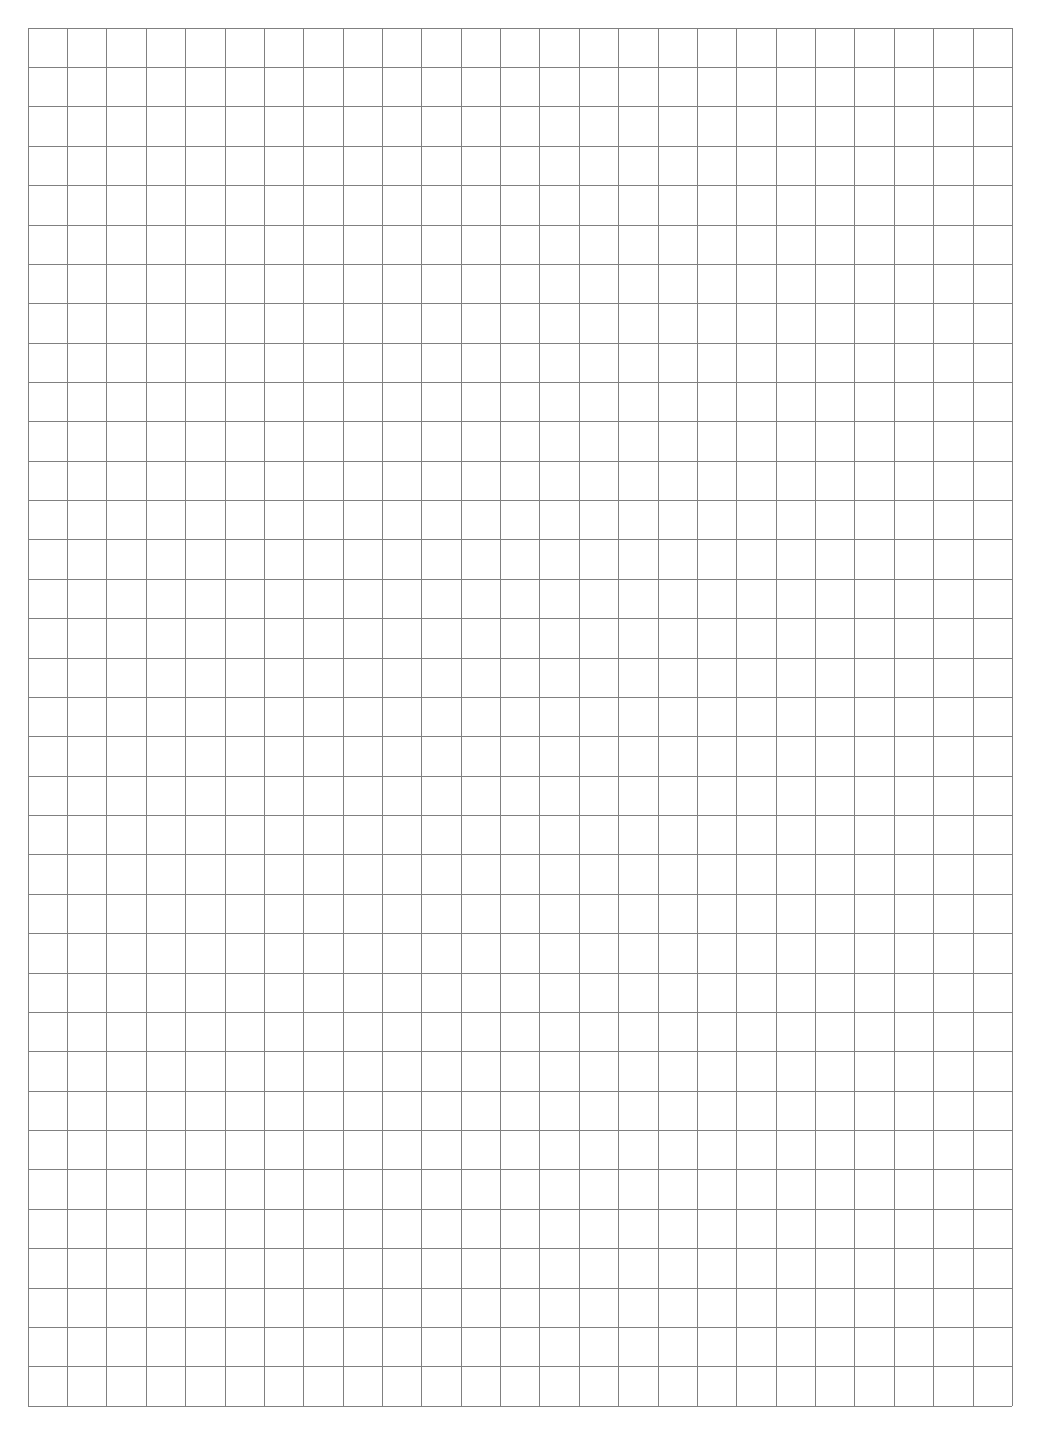
\begin{tikzpicture}[scale=.5]
\draw [very thin, gray] (0,0) grid (25,35);
  \end{tikzpicture}
\pagebreak
}
\rpt[10]{
 \section{blank}
\pagebreak
}


\rpt[4]{
\begin{figure}[p]
\centering
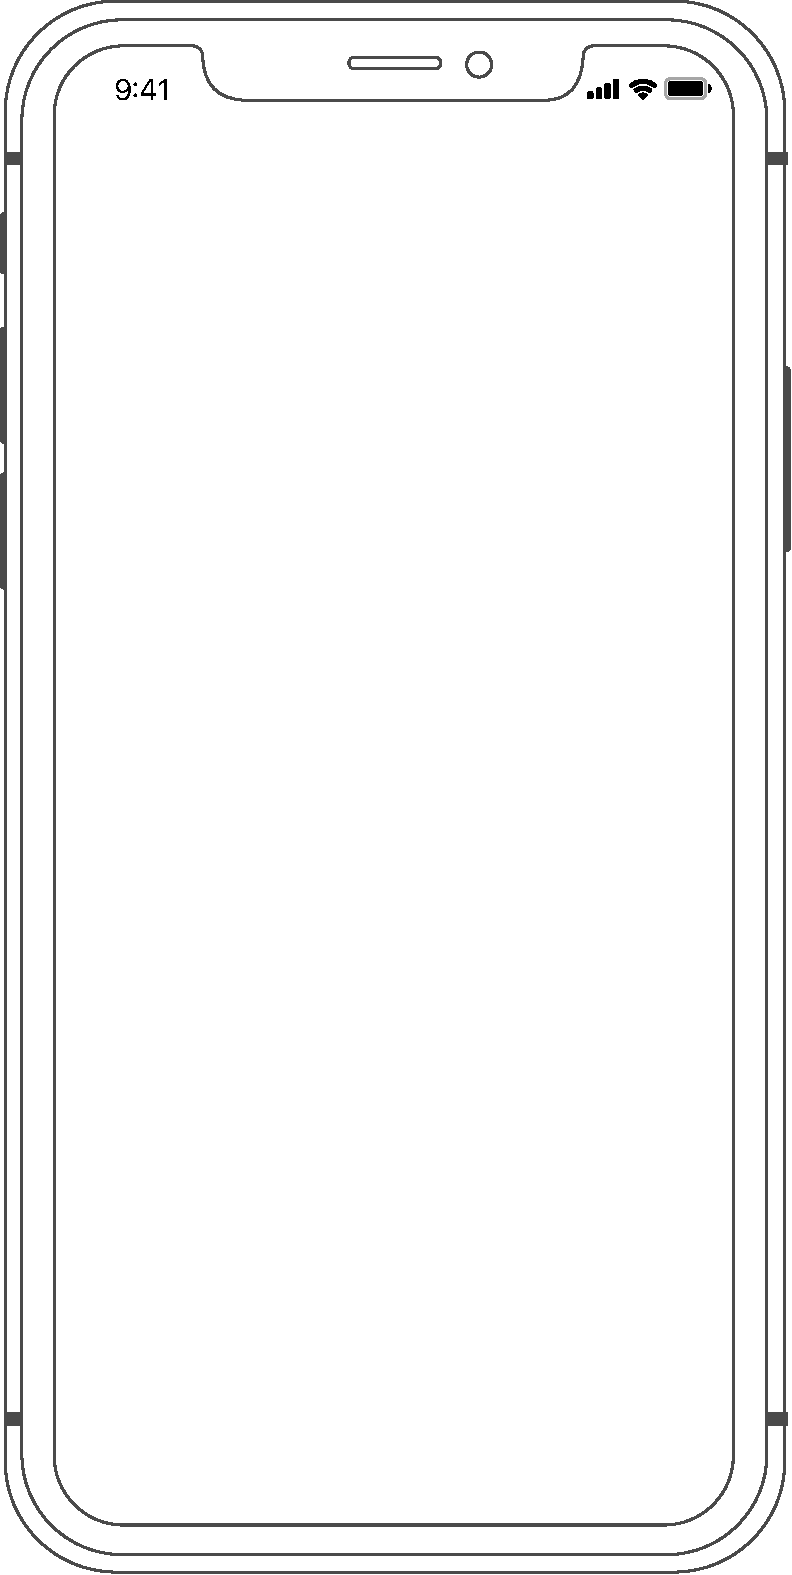
\includegraphics[height=143.6mm]{artwork/iPhoneX}
\end{figure}
\pagebreak
}

\begin{figure}[!h]
\centering
\begin{sideways}
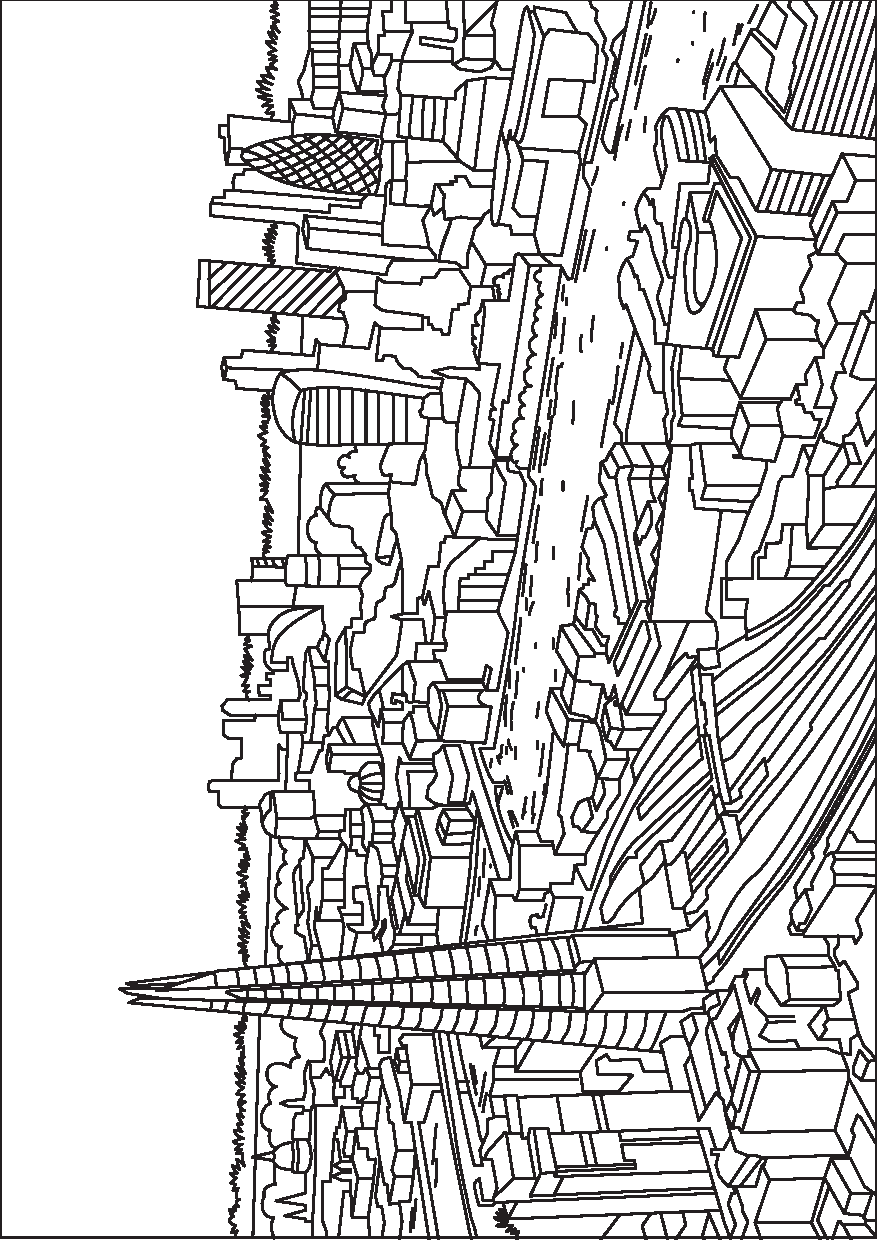
\includegraphics{./artwork/london}
\end{sideways}
\end{figure}
\pagebreak
\begin{figure}[!h]
\centering
\begin{sideways}
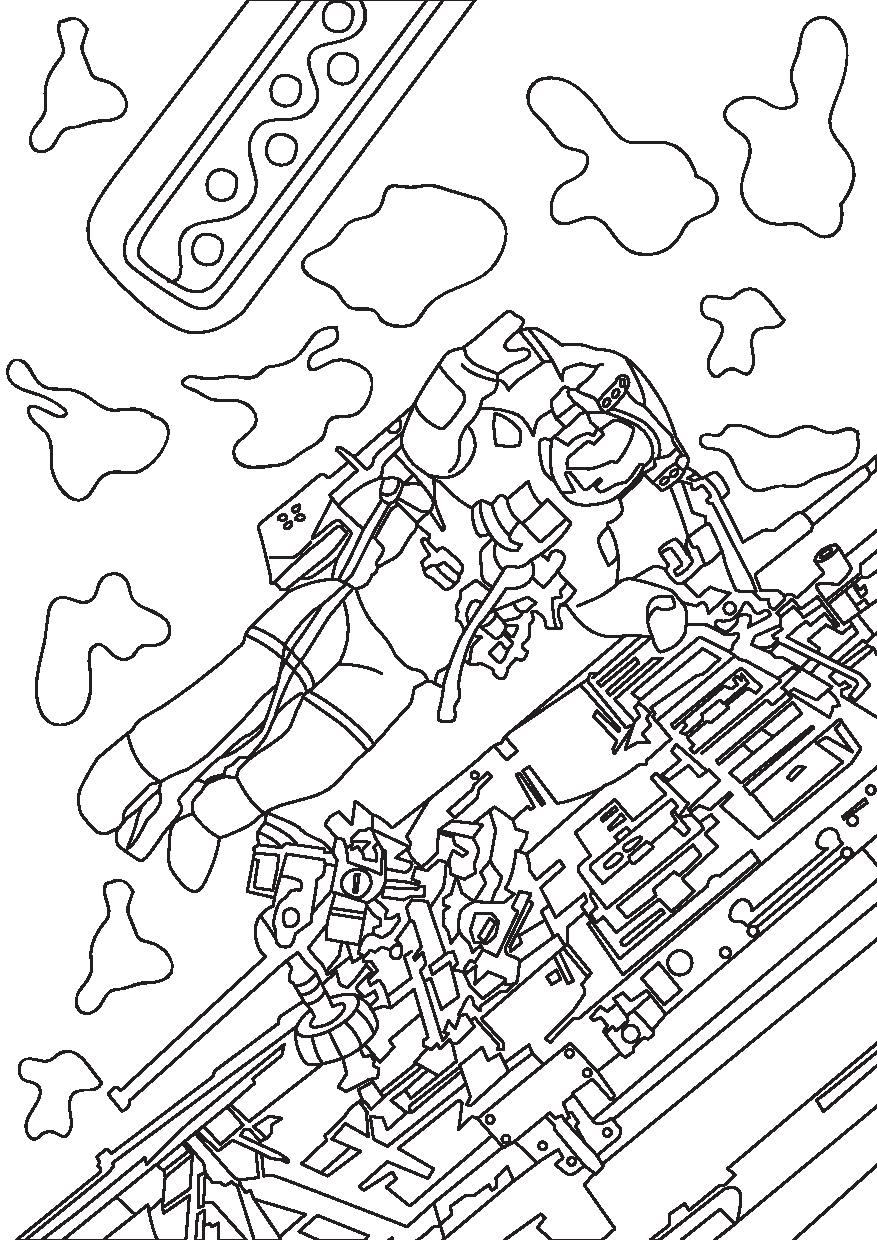
\includegraphics{./artwork/space}
\end{sideways}
\end{figure}
\pagebreak
\begin{figure}[!h]
\centering
\begin{sideways}
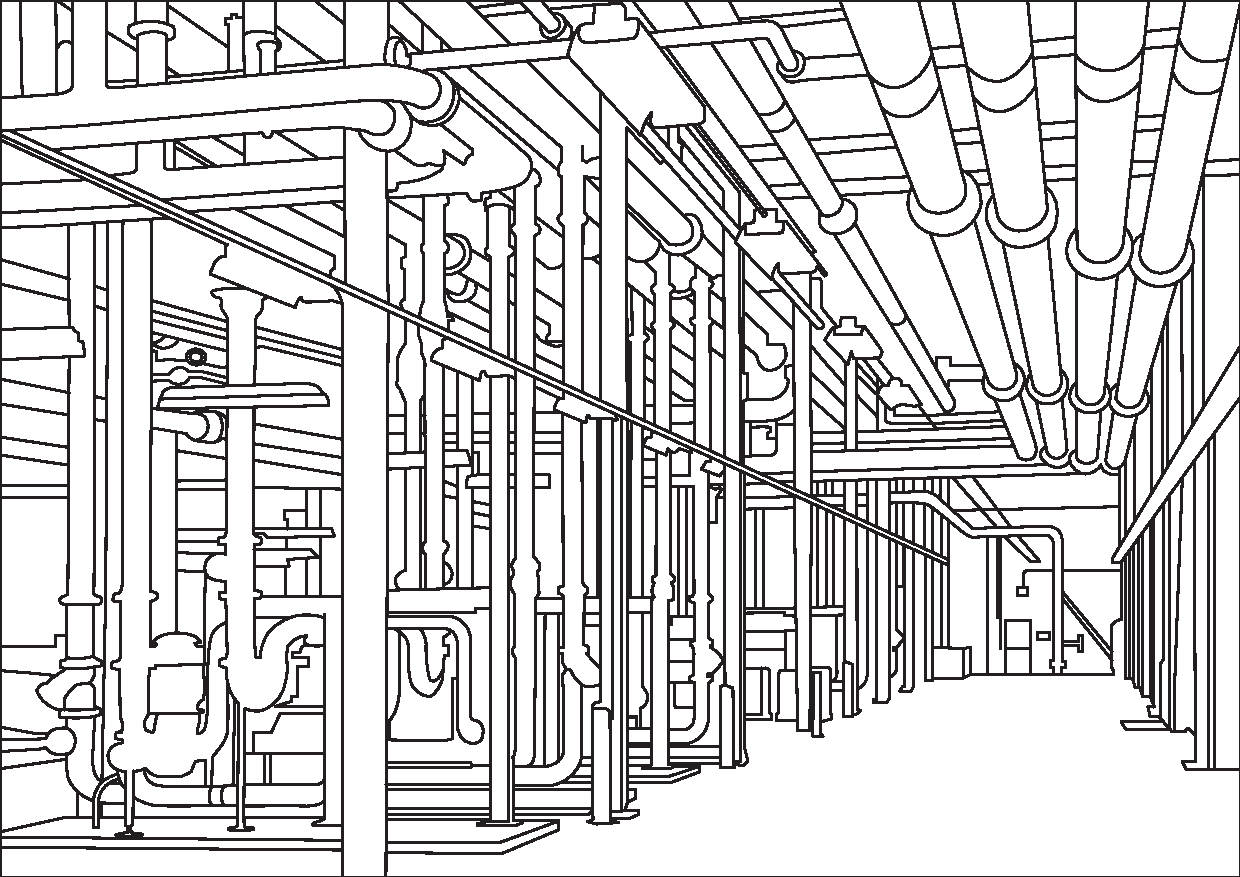
\includegraphics{./artwork/data_center}
\end{sideways}
\end{figure}
\pagebreak
%\documentclass{article}
%\usepackage{siunitx}
%\usepackage[sfdefault]{roboto}
%\usepackage[T1]{fontenc}

%\begin{document}

\begin{table}[p]
  \centering
  \begin{tabular}{l c c l}
   & Symbol & Value & SI unit \\
  \hline
  \\
  Planck constant & h & \num{6.62618e-34} & \si{\joule\second} \\
  \multicolumn{4}{l}{\textit{energy of a quantum of electromagnetic radiation / its frequency}} \\
  \\
  Electron mass & \si{\electronmass} & \num{9.10938e-31} & \si{\kilogram} \\
  \multicolumn{4}{l}{\textit{mass of a stationary electron}} \\
  \\
  Atomic mass unit (Dalton) & \si{\atomicmassunit} (\si{\dalton}) & \num{1.660566e-27} & \si{\kilogram} \\
  \multicolumn{4}{l}{\textit{one twelfth of the mass of an unbound neutral atom of carbon-12}} \\
  \\
  Elementary charge & \si{\elementarycharge} & \num{1.60218e-19} & \si{\coulomb} \\
  \multicolumn{4}{l}{\textit{electric charge carried by a single proton}} \\
  Electronvolt & \si{\electronvolt} & \num{1.60218e-19} & \si{\joule} \\
  \multicolumn{4}{l}{\textit{energy gained by charge of electron thru potential difference of one volt}} \\
  \\
  Bohr radius & \si{\bohr} & \num{5.29177e-11} & \si{\metre} \\
  \multicolumn{4}{l}{\textit{distance between the proton and electron in a hydrogen atom}} \\
  \\
  Faraday constant & F & \num{9.6485e4} & \si{\coulomb\per\mole} \\
  \multicolumn{4}{l}{\textit{magnitude of electric charge per mole of electrons}} \\
  \\
  Speed of light in a vacuum & \si{\clight} & \num{2.997925e8} & \si{\metre\per\second} \\
  \\
  Astronomical unit & \si{\astronomicalunit} & \num{1.49598e11} & \si{\metre} \\
  \multicolumn{4}{l}{\textit{roughly the distance from Earth to the Sun}} \\
  \\
  Avogadro number & \(N_{A}\) & \num{6.02204e23} & \si{\per\mole} \\
  \multicolumn{4}{l}{\textit{atoms or molecules in a mole}} \\
  \\
  \end{tabular}
  \caption{Some Fundamental Constants}
  \label{tab:constants}
\end{table}

%\end{document}
%\documentclass{article}
%\usepackage{siunitx}
%\usepackage[sfdefault]{roboto}
%\usepackage[T1]{fontenc}
%\usepackage{pifont}
%\usepackage{rotating}
%\begin{document}


\begin{table}[tbp]
  \centering
\begin{sideways}
%\resizebox{\textwidth}{!}{
%\tiny
\newcolumntype{R}{>{\ttfamily}r}
\begin{tabular}{ R @{\hskip 4pt}R @{\hskip 10pt}l @{\hskip 4pt}| @{\hskip 4pt}R @{\hskip 4pt}R @{\hskip 10pt}l @{\hskip 4pt}| @{\hskip 4pt}R @{\hskip 4pt}R @{\hskip 10pt}l @{\hskip 4pt}| @{\hskip 4pt}R @{\hskip 4pt}R @{\hskip 10pt}l }
Dec & Hex & \ttfamily Char                        & Dec & Hex & \ttfamily Char & Dec & Hex & \ttfamily Char & Dec & Hex & \ttfamily Char \\
\hline
0  &  0 & NUL (null)                    & 32 & 20 & Space  & 64 & 40 & @ & 96  & 60 & ` \\
1  &  1 & SOH (start of heading)        & 33 & 21 & !      & 65 & 41 & A & 97  & 61 & a \\
2  &  2 & STX (start of text)           & 34 & 22 & "      & 66 & 42 & B & 98  & 62 & b \\
3  &  3 & ETX (end of text)             & 35 & 23 & \#     & 67 & 43 & C & 99  & 63 & c \\
4  &  4 & EOT (end of transmission)     & 36 & 24 & \$     & 68 & 44 & D & 100 & 64 & d \\
5  &  5 & ENQ (enquiry)                 & 37 & 25 & \%     & 69 & 45 & E & 101 & 65 & e \\
6  &  6 & ACK (acknowledge)             & 38 & 26 & \&     & 70 & 46 & F & 102 & 66 & f \\
7  &  7 & BEL (bell)                    & 39 & 27 & '      & 71 & 47 & G & 103 & 67 & g \\
8  &  8 & BS (backspace)                & 40 & 28 & (      & 72 & 48 & H & 104 & 68 & h \\
9  &  9 & TAB (horizontal tab)          & 41 & 29 & )      & 73 & 49 & I & 105 & 69 & i \\
10 &  A & LF (line feed)                & 42 & 2A & *      & 74 & 4A & J & 106 & 6A & j \\
11 &  B & VT (vertical tab)             & 43 & 2B & +      & 75 & 4B & K & 107 & 6B & k \\
12 &  C & FF (form feed)                & 44 & 2C & ,      & 76 & 4C & L & 108 & 6C & l \\
13 &  D & CR (carriage return)          & 45 & 2D & -      & 77 & 4D & M & 109 & 6D & m \\
14 &  E & SO (shift out)                & 46 & 2E & .      & 78 & 4E & N & 110 & 6E & n \\
15 &  F & SI (shift in)                 & 47 & 2F & /      & 79 & 4F & O & 111 & 6F & o \\
16 & 10 & DLE (data link escape)        & 48 & 30 & 0      & 80 & 50 & P & 112 & 70 & p \\
17 & 11 & DC1 (device control 1)        & 49 & 31 & 1      & 81 & 51 & Q & 113 & 71 & q \\
18 & 12 & DC2 (device control 2)        & 50 & 32 & 2      & 82 & 52 & R & 114 & 72 & r \\
19 & 13 & DC3 (device control 3)        & 51 & 33 & 3      & 83 & 53 & S & 115 & 73 & s \\
20 & 14 & DC4 (device control 4)        & 52 & 34 & 4      & 84 & 54 & T & 116 & 74 & t \\
21 & 15 & NAK (negative acknowledge)    & 53 & 35 & 5      & 85 & 55 & U & 117 & 75 & u \\
22 & 16 & SYN (synchronous idle)        & 54 & 36 & 6      & 86 & 56 & V & 118 & 76 & v \\
23 & 17 & ETB (end of trans. block)     & 55 & 37 & 7      & 87 & 57 & W & 119 & 77 & w \\
24 & 18 & CAN (cancel)                  & 56 & 38 & 8      & 88 & 58 & X & 120 & 78 & x \\
25 & 19 & EM (end of medium)            & 57 & 39 & 9      & 89 & 59 & Y & 121 & 79 & y \\
26 & 1A & SUB (substitute)              & 58 & 3A & :      & 90 & 5A & Z & 122 & 7A & z \\
27 & 1B & ESC (escape)                  & 59 & 3B & ;      & 91 & 5B & [ & 123 & 7B & \{ \\
28 & 1C & FS (file separator)           & 60 & 3C & <      & 92 & 5C & \textbackslash & 124 & 7C & | \\
29 & 1D & GS (group separator)          & 61 & 3D & =      & 93 & 5D & ] & 125 & 7D & \} \\
30 & 1E & RS (record separator)         & 62 & 3E & >      & 94 & 5E & \textasciicircum & 126 & 7E & \textasciitilde \\
31 & 1F & US (unit separator)           & 63 & 3F & ?      & 95 & 5F & \_ & 127 & 7F & DEL \\

  \end{tabular}
%  }
  \end{sideways}
  \caption[]{\tabular[t]{@{}l@{}}ASCII Characters\endtabular}
  \label{tab:ascii}
\end{table}


%\end{document}


\begin{table}[tbp]
  \centering
\begin{tabular}{ l r }
Operation & Latency in nanoseconds \\
\hline
L1 cache reference & 0.5 ns \\
Branch mispredict & 5 ns \\
L2 cache reference & 7 ns \\
Main memory reference & 100 ns \\
Send 2K bytes over 1 Gbps network & 20,000 ns \\
Read 1 MB sequentially from memory & 250,000 ns \\
Round trip within same datacenter & 500,000 ns \\
Disk seek & 10,000,000 ns \\
Read 1 MB sequentially from disk & 20,000,000 ns \\
Send packet California->Europe->California & 150,000,000 ns
\end{tabular}
  
  \caption{Latency of key compute operations}
  \label{tab:numbers}
\end{table}

\newcolumntype{C}{>{\centering\arraybackslash}p{2.5em}}
\newcolumntype{L}{>{\arraybackslash}p{7em}}

\begin{table}[tbp]
  \centering
\begin{tabular}{ L r C L r}
\multicolumn{5}{c}{Countries by population} \\
\hline
China & 1,376 & & Mexico & 122\\
India & 1,288 & & Philippines & 103\\
United States & 323 & & Ethiopia & 92\\
Indonesia & 259 & & Vietnam & 92 \\
Brazil & 206 & & Egypt & 91\\
Pakistan & 193 & & DR Congo & 85 \\
Nigeria & 187 & & Germany & 81 \\
Bangladesh & 160 & & Iran & 79 \\
Russia & 147 & & Turkey & 79\\
Japan & 127 & & Thailand & 65
\end{tabular}
  
  \caption{Population data: 100,000s 2016}
  \label{tab:numbers}
\end{table}


\end{document}
